\section{Results}
\label{sec:result}

Our algorithm is tested on a variety of 3D shapes. 
We visualize the discrete matches using the similar color as the corresponding symmetry parts.

We first show experimental results on clean manifold meshes, which are not corrupted with noise, and are complete. 
For such models, our algorithm provides good segmentation for the partial matching, and we reliably obtain perfect results (e.g. Figure~\ref{fig:Eager} and~\ref{fig:Tiger}). 

\begin{figure}[t]
\centering
  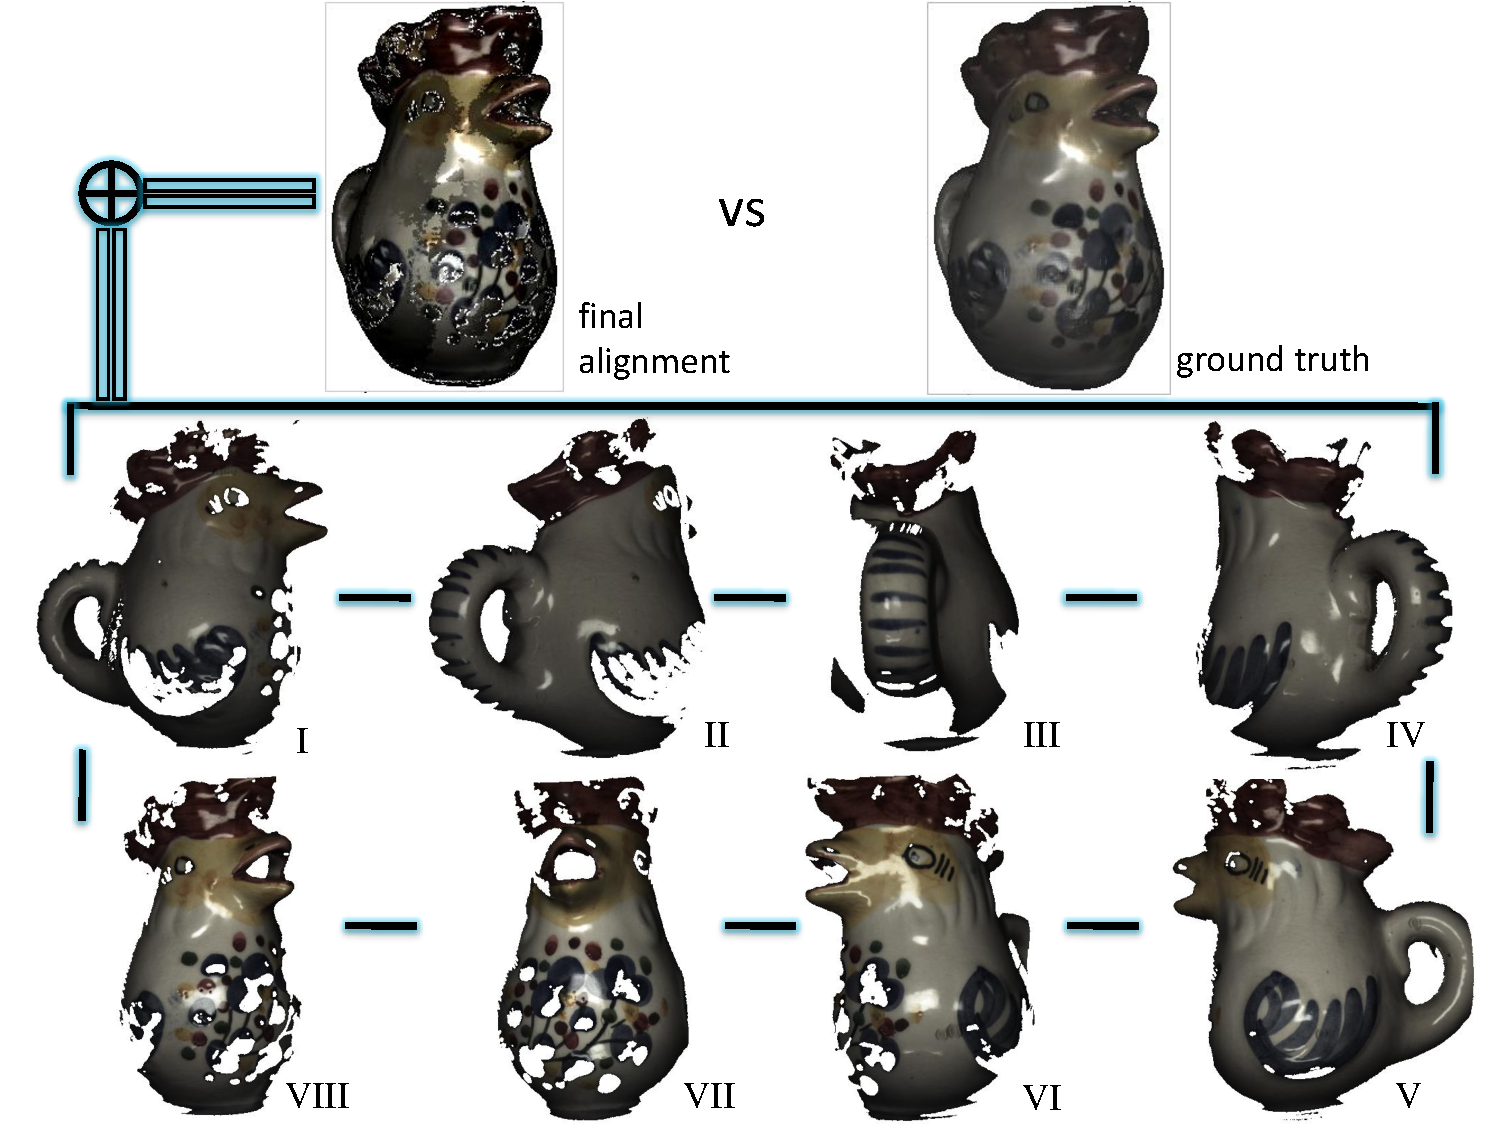
\includegraphics[width=0.99\linewidth]{figures/Rooster.pdf}
  \caption{The four legs could be detected as one symmetric region at the current configuration $c=0.2/n$.
  It is mainly resulting from the large similarity of four legs.}
\label{fig:Tiger}
\end{figure}

As our algorithm works on the meaningful segmentation, uniform sampling, and clustering, the matching results do not depend on the tessellation of the shapes.
Figure~\ref{fig:Point} demonstrates that our algorithm performs very well on the shape in the point set form.

\begin{figure}[t]
\centering
  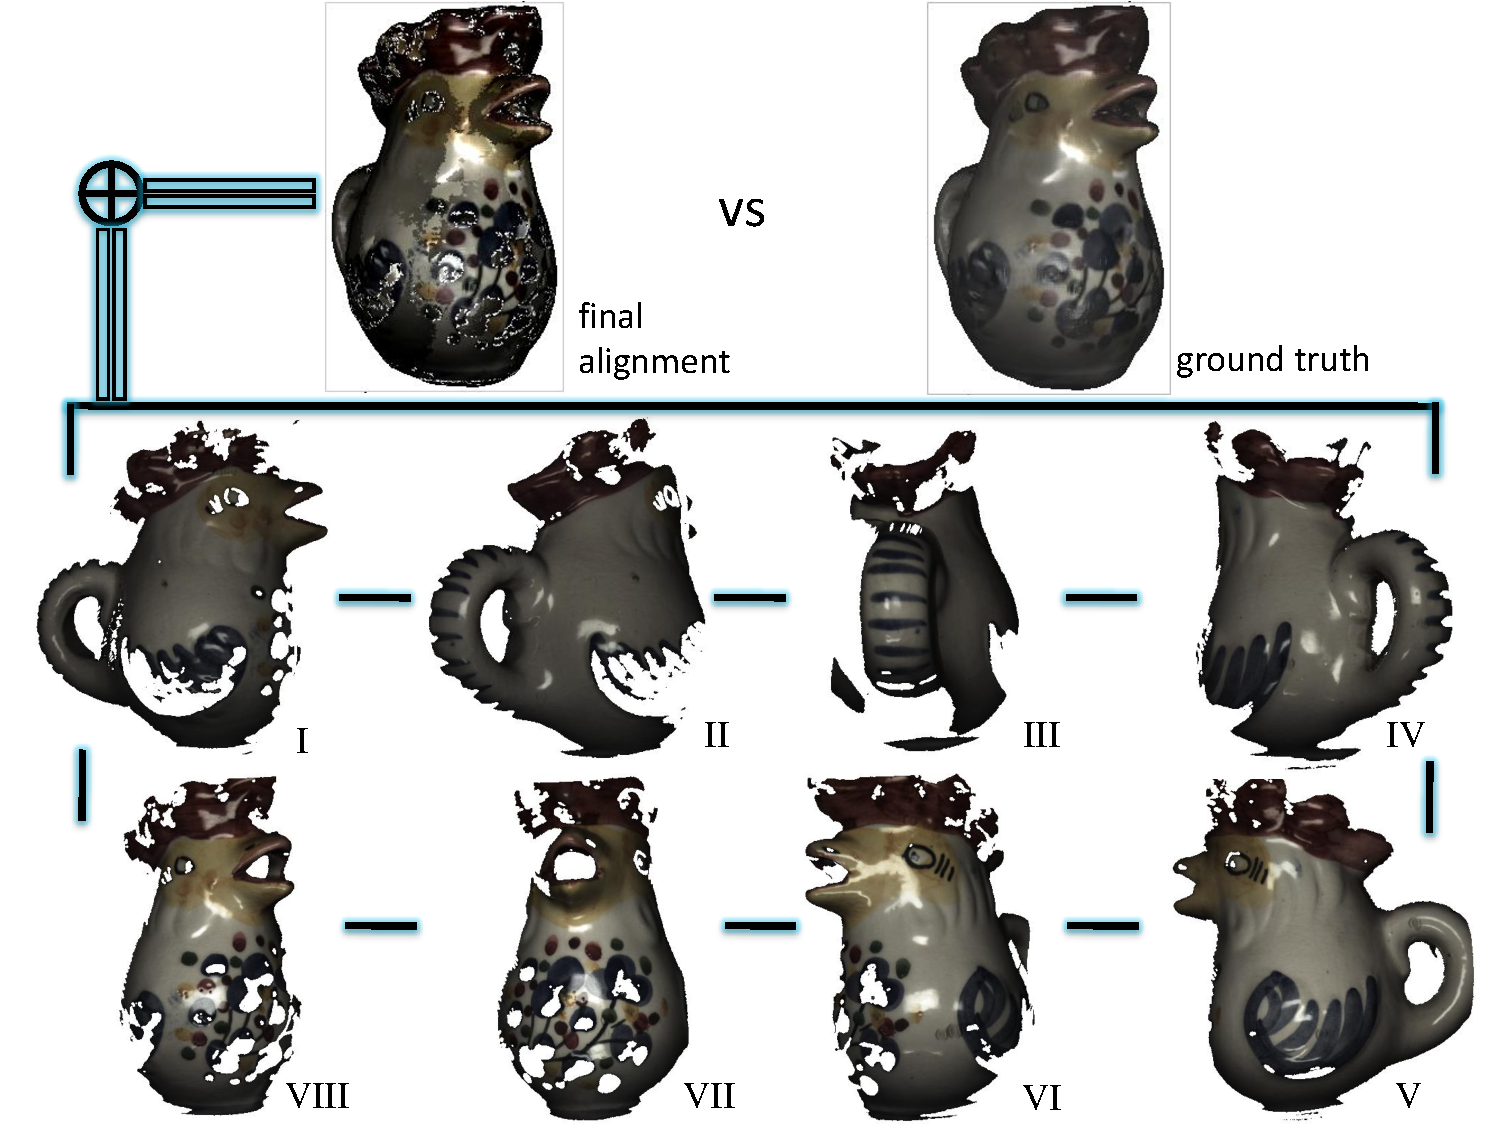
\includegraphics[width=0.99\linewidth]{figures/Rooster.pdf}
  \caption{The in point set form.}
\label{fig:Point}
\end{figure}

Figure~\ref{fig:Gargoyl} shows an example using the three different symmetry group composed of reflection, rotation, and translation.
The symmetry is detected in coarse-to-fine steps based on the hierarchical segmentation.
In the coarse level, all major reflection symmetries are faithfully recovered.
While in the fine level, most rotation and translation symmetries are detected.
Note that, the example is clearly claimed as the failure case in the STAR algorithm~\cite{berner2011}.

We use another example on the complete and non-complete Armidillo (Figure~\ref{fig:Arm}) to demonstrate the robustness of our algorithm.
Both on the complete and non-complete cases, the algorithm computes a global reflectional plane based on all final correspondences. 
Experiments show that the plane is almost same in the both cases.

\begin{figure}[t]
\centering
  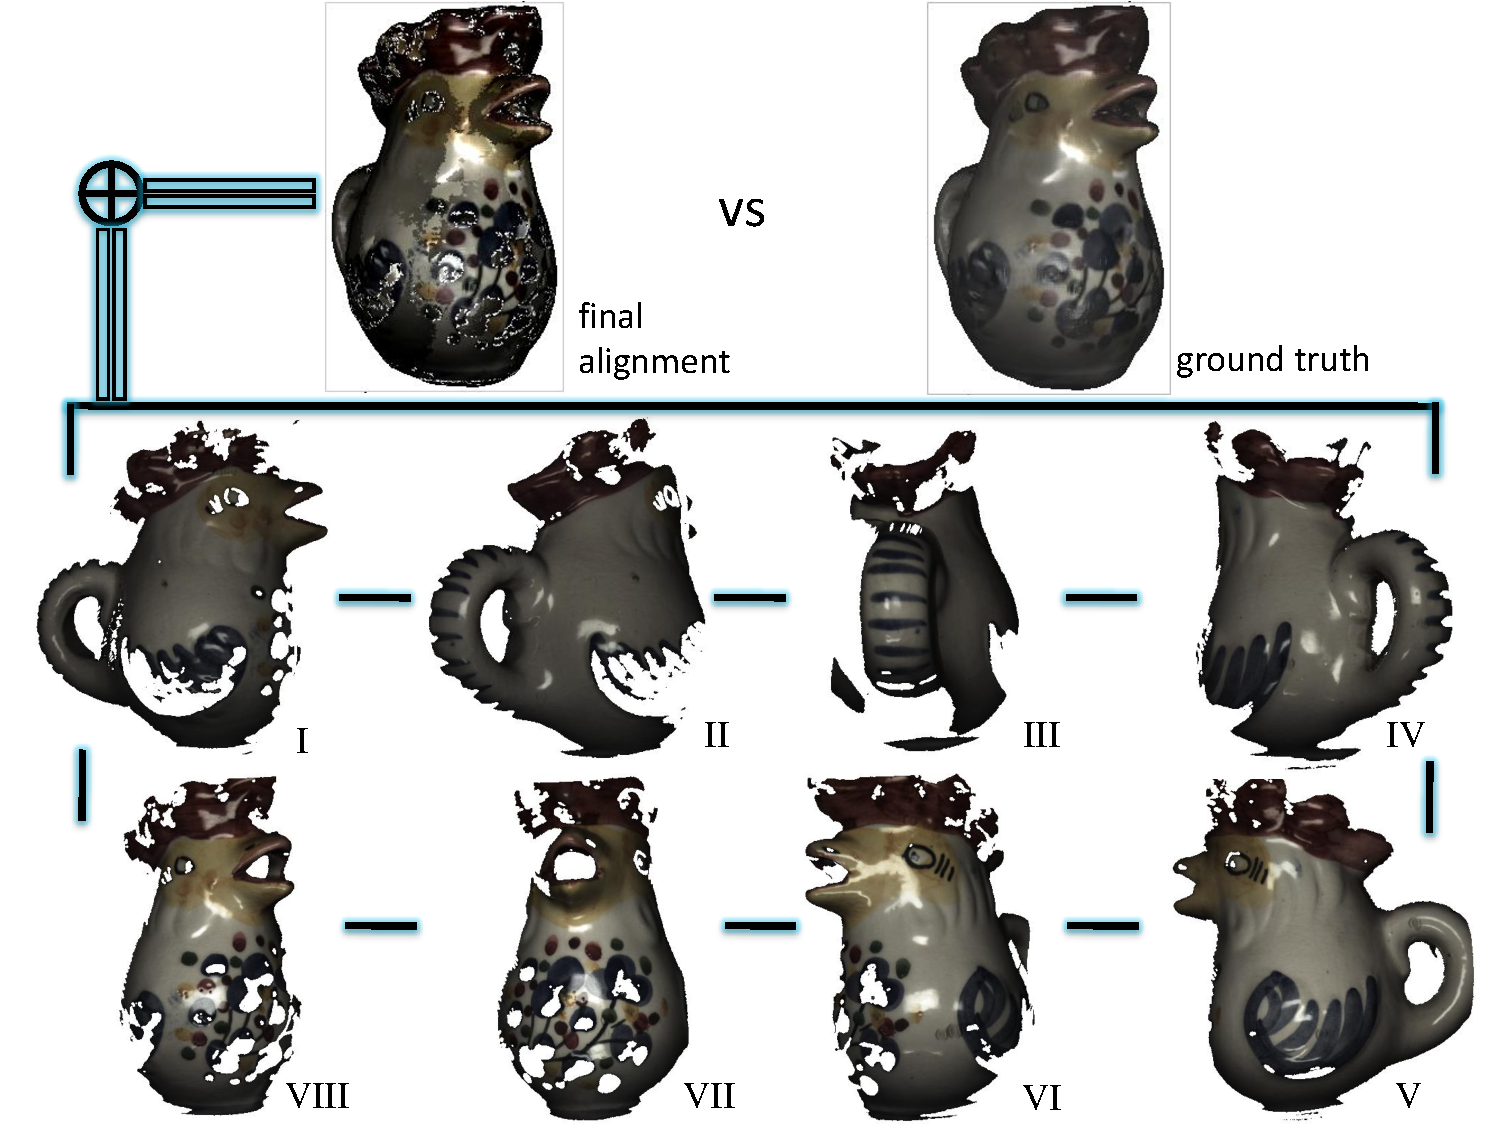
\includegraphics[width=0.99\linewidth]{figures/Rooster.pdf}
  \caption{The global reflectional planes are computed from the complete and non-complete Armadillo shapes.}
\label{fig:Arm}
\end{figure}

The performance data of Table 1 indicates how the computation on the symmetries of the shapes.

\begin{table*}
\centering
\begin{tabular}{l|r|r|r|r|r}
Model
& Vertices
& Parts number
& Segmentation
& Partial matching
& Correspondences clustering \\
\hline
%%%RRM Use captial letter for all model names
Armadillo  & 172,974  & 9 &  982ms   & 2ms & 7ms \\
bumpy plane&   3,721  & 14 & 47ms     & 1ms & 2ms  \\
Eager      &  14,618  & 6 & 413ms    & 2ms & 3ms \\
Gargoyl    & 250,003  & 6 & 218ms    & 3ms & 3ms  \\
%feline     &  49,864  & 20 & 109ms    & 3ms & 2ms \\

\hline
\end{tabular}
\caption{Timing for our algorithm: automatic meaningful segmentation, partial matching of each part,
and clustering the correspondences, using a 1.6GHz Intel Core i7CPU laptop with 4GB of RAM.
}
\label{tab:timing}
\end{table*}